\documentclass[]{../common/elementary-physics}

\title{4. Increasing Magnetic Flux}
\date{2015-05-27 v0.9}

\begin{document}

\maketitle

\tableofcontents

\section{Abstract}

By using the template in our third paper\cite{analogies} it becomes easy to make a template for the 'elastic collision' and then show if magnetic flux increase in a $CLL$-system.

\section{The Template}

The template assumes a lossless system:

\begin{align}
a y'' + b y' + c y &= 0 \\
a &> 0 \\
b &= 0 \\
c &= c_1 + c_2 \\
a y'' + (c_1 + c_2) y &= 0 \\
y_0 &= \frac{z_1-z_2}{c} \\
y'_0 &= 0 \\
y &= y_0 \, cos(\sqrt{\frac{c}{a} \, t})
\end{align}

At $t=0$ the 'elastic collision' begins and $y=y_0$.
At $t = \pi \, \sqrt{\frac{a}{c}}$ it is completed and $y = -y_0$, therefore the template is:

\begin{align}
y_0 &= \frac{{z_1}_{old}-{z_2}_{old}}{c_1 + c_2} \\
{y_1}_{old} &= \frac{{z_1}_{old}}{c_1} \\
{y_2}_{old} &= \frac{{z_2}_{old}}{c_2} \\
{y_1}_{new} &= {y_1}_{old} -2 y_0 \\
{y_2}_{new} &= {y_2}_{old} +2 y_0 \\
{z_1}_{new} &= c_1 {y_1}_{new} \\
{z_2}_{new} &= c_2 {y_2}_{new}
\end{align}

Which corresponds to our previous paper\cite{masspar}.

If $c_1 > c_2$ and ${z_1}_{old} > 0$ then $\sum |y|$ will increase when ${y_1}_{old} < 2 y_0$.

\section{Increasing Absolute Momentum Revisited}

The system used is a lossless $kbm$\cite{analogies}: $k^{-1} p'' + (m_1^{-1} + m_2^{-1}) p = 0$.

\begin{figure}[ht] \centering
	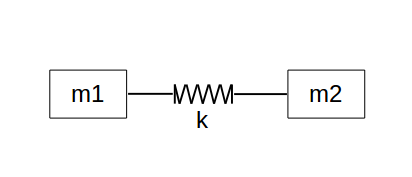
\includegraphics[scale=.3]{mkm} \caption{Transfer of momentum}
\end{figure}

From the template above we have:

\begin{align}
p_0 &= \frac{m_1 m_2 ({v_1}_{old}-{v_2}_{old})}{m_1 + m_2} \\
{p_1}_{old} &= m_1 {v_1}_{old} \\
{p_2}_{old} &= m_2 {v_2}_{old} \\
{p_1}_{new} &= {p_1}_{old} -2 p_0 \\
{p_2}_{new} &= {p_2}_{old} +2 p_0 \\
{v_1}_{new} &= \frac{{p_1}_{new}}{m_1} \\
{v_2}_{new} &= \frac{{p_2}_{new}}{m_2}
\end{align}

If $m_1 < m_2$ and ${v_1}_{old} > 0$ then $\sum |p|$ will increase when ${p_1}_{old} < 2 p_0$.
Let us reuse the example from the previous paper\cite{incmom}:

\begin{align}
m_1 &= 2 \, kg \\
v_1 &= 1 \, m/s \\
m_2 &= 3 \, kg \\
v_2 &= 0 \, m/s
\end{align}

And so:

\begin{align}
p_0 &= \frac{2 * 3 * (1-0)}{2 + 3} = \frac{6}{5} \, kg \, m/s \\
{p_1}_{old} &= 2 * 1 = 2 \, kg \, m/s \\
{p_2}_{old} &= 3 * 0 = 0 \, kg \, m/s \\
{p_1}_{new} &= 2 -2 * \frac{6}{5} = -\frac{2}{5} \, kg \, m/s \\
{p_2}_{new} &= 0 +2 * \frac{6}{5} = \frac{12}{5} \, kg \, m/s \\
{v_1}_{new} &= -\frac{\frac{2}{5}}{2} = -\frac{1}{5} \, m/s \\
{v_2}_{new} &= \frac{\frac{12}{5}}{3} = \frac{4}{5} \, m/s
\end{align}

$\sum |p|$ has increased from $2 \, kg \, m/s$ to $\frac{14}{5} = 2.8 \, kg \, m/s$.

\section{Increasing Absolute Charge Revisited}

The system used is a lossless $LRC$\cite{analogies}: $L Q'' + (C_1^{-1} + c_2^{-1}) Q = 0$.

\begin{figure}[ht] \centering
	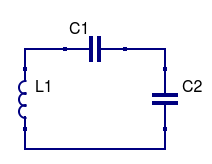
\includegraphics[scale=.5]{LCC} \caption{Transfer of charge}
\end{figure}

From the template above we have:

\begin{align}
Q_0 &= \frac{C_1 C_2 ({V_1}_{old}-{V_2}_{old})}{C_1 + C_2} \\
{Q_1}_{old} &= C_1 {V_1}_{old} \\
{Q_2}_{old} &= C_2 {V_2}_{old} \\
{Q_1}_{new} &= {Q_1}_{old} -2 Q_0 \\
{Q_2}_{new} &= {Q_2}_{old} +2 Q_0 \\
{V_1}_{new} &= \frac{{Q_1}_{new}}{C_1} \\
{V_2}_{new} &= \frac{{Q_2}_{new}}{C_2}
\end{align}

If $C_1 < C_2$ and ${V_1}_{old} > 0$ then $\sum |Q|$ will increase when ${Q_1}_{old} < 2 Q_0$.
Let us reuse the example from the previous paper\cite{incmom}:

\begin{align}
C_1 &= 2 \, F \\
V_1 &= 1 \, V \\
C_2 &= 3 \, F \\
V_2 &= 0 \, V
\end{align}

And so:

\begin{align}
Q_0 &= \frac{2 * 3 * (1-0)}{2 + 3} = \frac{6}{5} \, C \\
{Q_1}_{old} &= 2 * 1 = 2 \, C \\
{Q_2}_{old} &= 3 * 0 = 0 \, C \\
{Q_1}_{new} &= 2 -2 * \frac{6}{5} = -\frac{2}{5} \, C \\
{Q_2}_{new} &= 0 +2 * \frac{6}{5} = \frac{12}{5} \, C \\
{V_1}_{new} &= -\frac{\frac{2}{5}}{2} = -\frac{1}{5} \, V \\
{V_2}_{new} &= \frac{\frac{12}{5}}{3} = \frac{4}{5} \, V
\end{align}

$\sum |Q|$ has increased from $2 \, C$ to $\frac{14}{5} = 2.8 \, C$.

\section{Increasing Absolute Distance}

The system used is a lossless $mbk$\cite{analogies}: $m x'' + (k_1 + k_2) x = 0$.

\begin{figure}[ht] \centering
	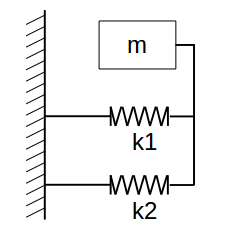
\includegraphics[scale=.3]{kmk} \caption{Transfer of distance}
\end{figure}

From the template above we have:

\begin{align}
x_0 &= \frac{{F_1}_{old}-{F_2}_{old}}{k_1 + k_2} \\
{x_1}_{old} &= \frac{{F_1}_{old}}{k_1} \\
{x_2}_{old} &= \frac{{F_2}_{old}}{k_2} \\
{x_1}_{new} &= {x_1}_{old} -2 x_0 \\
{x_2}_{new} &= {x_2}_{old} +2 x_0 \\
{F_1}_{new} &= k_1 {x_1}_{new} \\
{F_2}_{new} &= k_2 {x_2}_{new}
\end{align}

If $k_1 > k_2$ and ${F_1}_{old} > 0$ then $\sum |x|$ will increase when ${x_1}_{old} < 2 x_0$.
Let us reuse the numbers from the previous paper\cite{incmom}:

\begin{align}
k_1 &= \frac{1}{2} \, N/m \\
F_1 &= 1 \, N \\
k_2 &= \frac{1}{3} \, N/m \\
F_2 &= 0 \, N
\end{align}

And so:

\begin{align}
x_0 &= \frac{1-0}{\frac{1}{2} + \frac{1}{3}} = \frac{6}{5} \, m \\
{x_1}_{old} &= \frac{1}{\frac{1}{2}} = 2 \, m \\
{x_2}_{old} &= \frac{0}{\frac{1}{3}} = 0 \, m \\
{x_1}_{new} &= 2 -2 * \frac{6}{5} = -\frac{2}{5} \, m \\
{x_2}_{new} &= 0 +2 * \frac{6}{5} = \frac{12}{5} \, m \\
{F_1}_{new} &= - \frac{1}{2} * \frac{2}{5} = -\frac{1}{5} \, N \\
{F_2}_{new} &= \frac{1}{3} * \frac{12}{5} = \frac{4}{5} \, N
\end{align}

$\sum |x|$ has increased from $2 \, m$ to $\frac{14}{5} = 2.8 \, m$ where $x$ is the offset from where the spring exerts no force.

\section{Increasing Absolute Magnetic Flux Linkage}

The system used is a lossless $CRL$\cite{analogies}: $C \Lambda'' + (L_1^{-1} + L_2^{-1}) \Lambda = 0$ where $\Lambda = \Phi N$ and is referred to as magnetic flux linkage.

\begin{figure}[ht] \centering
	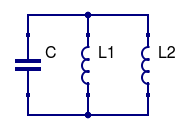
\includegraphics[scale=.5]{CLL} \caption{Transfer of magnetic flux linkage}
\end{figure}

From the template above we have:

\begin{align}
\Lambda_0 &= \frac{L_1 L_2 ({I_1}_{old}-{I_2}_{old})}{L_1 + L_2} \\
{\Lambda_1}_{old} &= L_1 {I_1}_{old} \\
{\Lambda_2}_{old} &= L_2 {I_2}_{old} \\
{\Lambda_1}_{new} &= {\Lambda_1}_{old} -2 \Lambda_0 \\
{\Lambda_2}_{new} &= {\Lambda_2}_{old} +2 \Lambda_0 \\
{I_1}_{new} &= \frac{{\Lambda_1}_{new}}{L_1} \\
{I_2}_{new} &= \frac{{\Lambda_2}_{new}}{L_2}
\end{align}

If $L_1 < L_2$ and ${I_1}_{old} > 0$ then $\sum |\Lambda|$ will increase when ${\Lambda_1}_{old} < 2 \Lambda_0$.
Let us reuse the numbers from the previous paper\cite{incmom}:

\begin{align}
L_1 &= 2 \, H \\
I_1 &= 1 \, A \\
L_2 &= 3 \, H \\
I_2 &= 0 \, A
\end{align}

And so:

\begin{align}
\Lambda_0 &= \frac{2 * 3 * (1-0)}{2 + 3} = \frac{6}{5} \, Wb \\
{\Lambda_1}_{old} &= 2 * 1 = 2 \, Wb \\
{\Lambda_2}_{old} &= 3 * 0 = 0 \, Wb \\
{\Lambda_1}_{new} &= 2 -2 * \frac{6}{5} = -\frac{2}{5} \, Wb \\
{\Lambda_2}_{new} &= 0 +2 * \frac{6}{5} = \frac{12}{5} \, Wb \\
{I_1}_{new} &= -\frac{\frac{2}{5}}{2} = -\frac{1}{5} \, A \\
{I_2}_{new} &= \frac{\frac{12}{5}}{3} = \frac{4}{5} \, A
\end{align}

$\sum |\Lambda|$ has increased from $2 \, Wb$ to $\frac{14}{5} = 2.8 \, Wb$.
But remember that $\Lambda = \Phi N$ so what happened to the flux $\Phi$ without the linkage $N$?

$A_L$ is frequently specified by transformer-core manufacturers and is defined as:

\begin{equation}
A_L = \frac{L}{N^2}
\end{equation}

It can be used for any coil.
As an example, for a multilayer air-core coil\cite{wpind}:

\begin{align}
L &= \frac{4}{5} \frac{r^2 N^2}{6r+9l+10d} \\
A_L &= \frac{4}{5} \frac{r^2}{6r+9l+10d}
\end{align}

If we assume $A_{L_1} = A_{L_2}$ we can substitute $N = \sqrt{L/A_L}$ and calculate:

\begin{eqnarray}
\Lambda = \Phi N &=& \frac{\Phi \sqrt{L}}{\sqrt{A_L}} \\
\frac{\Lambda}{\sqrt{L}} = \frac{\Phi N}{\sqrt{L}} &=& \frac{\Phi}{\sqrt{A_L}}
\end{eqnarray}

which since $A_{L_1} = A_{L_2}$ will enable us to calculate:

\begin{align}
\frac{\sum |\Phi_{new}|}{\sum \Phi_{old}} = \frac{\sum |\Lambda_{new} / \sqrt{L}|}{\sum \Lambda_{old} / \sqrt{L}} = \frac{\frac{2}{5}/\sqrt{2}+\frac{12}{5}/\sqrt{3}}{2/\sqrt{2}}\approx 1.18
\end{align}

$\sum |\Phi|$ has increased by a factor $1.18$.
Let us also calculate:

\begin{align}
\frac{\sum \Phi_{new}}{\sum \Phi_{old}} = \frac{\sum \Lambda_{new} / \sqrt{L}}{\sum \Lambda_{old} / \sqrt{L}} = \frac{-\frac{2}{5}/\sqrt{2}+\frac{12}{5}/\sqrt{3}}{2/\sqrt{2}}\approx 0.78
\end{align}

$\sum \Phi$ has decreased by a factor $0.78$.

$\sum E$ is still constant and so is $\sum {\Phi}^2$.

Watch an excellent experiment by youtube user \textbf{gotoluc} that we believe is relevant in this context: \url{https://www.youtube.com/watch?v=XfLcBD3Fy7M}.

\section{Conclusion}

While $\sum y$ is always constant $\sum |y|$ is sometimes not, just as shown in our previous paper\cite{incmom} for momentum and charge.
When $y = \Lambda = \Phi N$, as in the $CRL$-system, not even $\sum \Phi$ has to be constant.

\appendix

\section{In Plain English}

In our previous paper\cite{incmom} we proposed a template for comparing different simple harmonic systems, their variables and equations.
In this paper, we compile a template to easily calculate the output of an elastic collision, and its equivalent in other systems.
Also the conditions under which the sum of the absolute value of the system's momentum is no longer constant can be calculated.
If the system comprises two coils and a capacitor in parallel, it is not just the sum of the absolute value of the magnetic fluxe linkages in the coils which may vary but also the sum of their magnetic fluxes.

\section{På Ren Svenska}

I vår förra artikel\cite{incmom} föreslog vi en schablon för att kunna jämföra olika enkla harmoniska system, deras variabler och ekvationer.
I denna artikel sammanställer vi en schablon för att enkelt kunna beräkna utgången av en elastisk kollision och dess motsvarighet i andra system.
Även villkoren för när summan av absolutvärdet av systemets rörelsemängd inte längre är konstant kan beräknas.
Om systemet består av två spolar och en kondensator parallellt är det inte bara summan av absolutvärdet av de magnetiska flödesbanden i spolarna som kan variera utan även summan av deras magnetiska flöden.

\section{This Paper}

This is one paper from a collection of papers, all free to be downloaded and shared. If you have ideas how to enhance any of the papers, if you want to contribute, don’t hesitate to contact us at \url{hob.nilre@gmail.com}.\\
\\
The papers can all be found at:
\begin{itemize}
\item \url{https://sites.google.com/site/nilrehob/home/elementary-physics}
\item \url{https://independent.academia.edu/HobNilre/Papers}
\item \url{https://groups.yahoo.com/neo/groups/EVGRAY/files/Hob/}
\item \url{http://overunity.com/15796/elementary-physics-revisited/}
\item \url{http://idipsum.se/home/elementary%20physics.html}
\item \url{https://github.com/boherlin/elementary-physics/tree/master/pdf}
\end{itemize}

They are updated with new versions in an unpredictable manner, possibly not on all sites but at least on the last two sites in the list, make sure you always have the latest version!
Their \LaTeX source-codes can be found at \url{https://github.com/boherlin/elementary-physics/tree/master/src}.
All papers, but not all versions, have been stamped at \url{http://www.OriginStamp.org}.\\
\\
If you enjoyed this paper, found value in it and want to help us, please consider giving us a donation in bitcoin, this is our address:

\begin{figure}[ht] \centering
	
\includegraphics[]{1B79p75vQw4Rb1GQdmGYpDapFwEytFJDqw} \caption{1B79p75vQw4Rb1GQdmGYpDapFwEytFJDqw}
\end{figure}


\printbibliography

\end{document}

